\section{Title2Rec}
\label{sec:t2r}
Title2Rec recommends tracks taking as input the playlist title, following the procedure illustrated in Figure~\ref{fig:t2r_rec}. The title is translated into a vector $p_{t2r}$, named title embedding, computed by applying the strategy described in Section~\ref{sec:title_embs} to the playlists defined in the MPD dataset.

Given a new seed playlist, we compute its title embedding in the same way. Then, we select a subset $P$ including the top-300 most similar playlists to the given one by comparing its embeddings with $p_{t2r}$ using the cosine similarity. Finally, the required number of tracks are selected among the ones available in $P$. The tracks have been ordered to ensure that the most popular ones in $P$ are placed at the top of the list.

% source https://docs.google.com/presentation/d/1KV4eFuYvFxS1Z25ZwOqu5TJ2zuBbeRAZAkR2Hbf8h_A/edit#slide=id.g3b0c032961_0_82
\begin{figure}
    \centering
    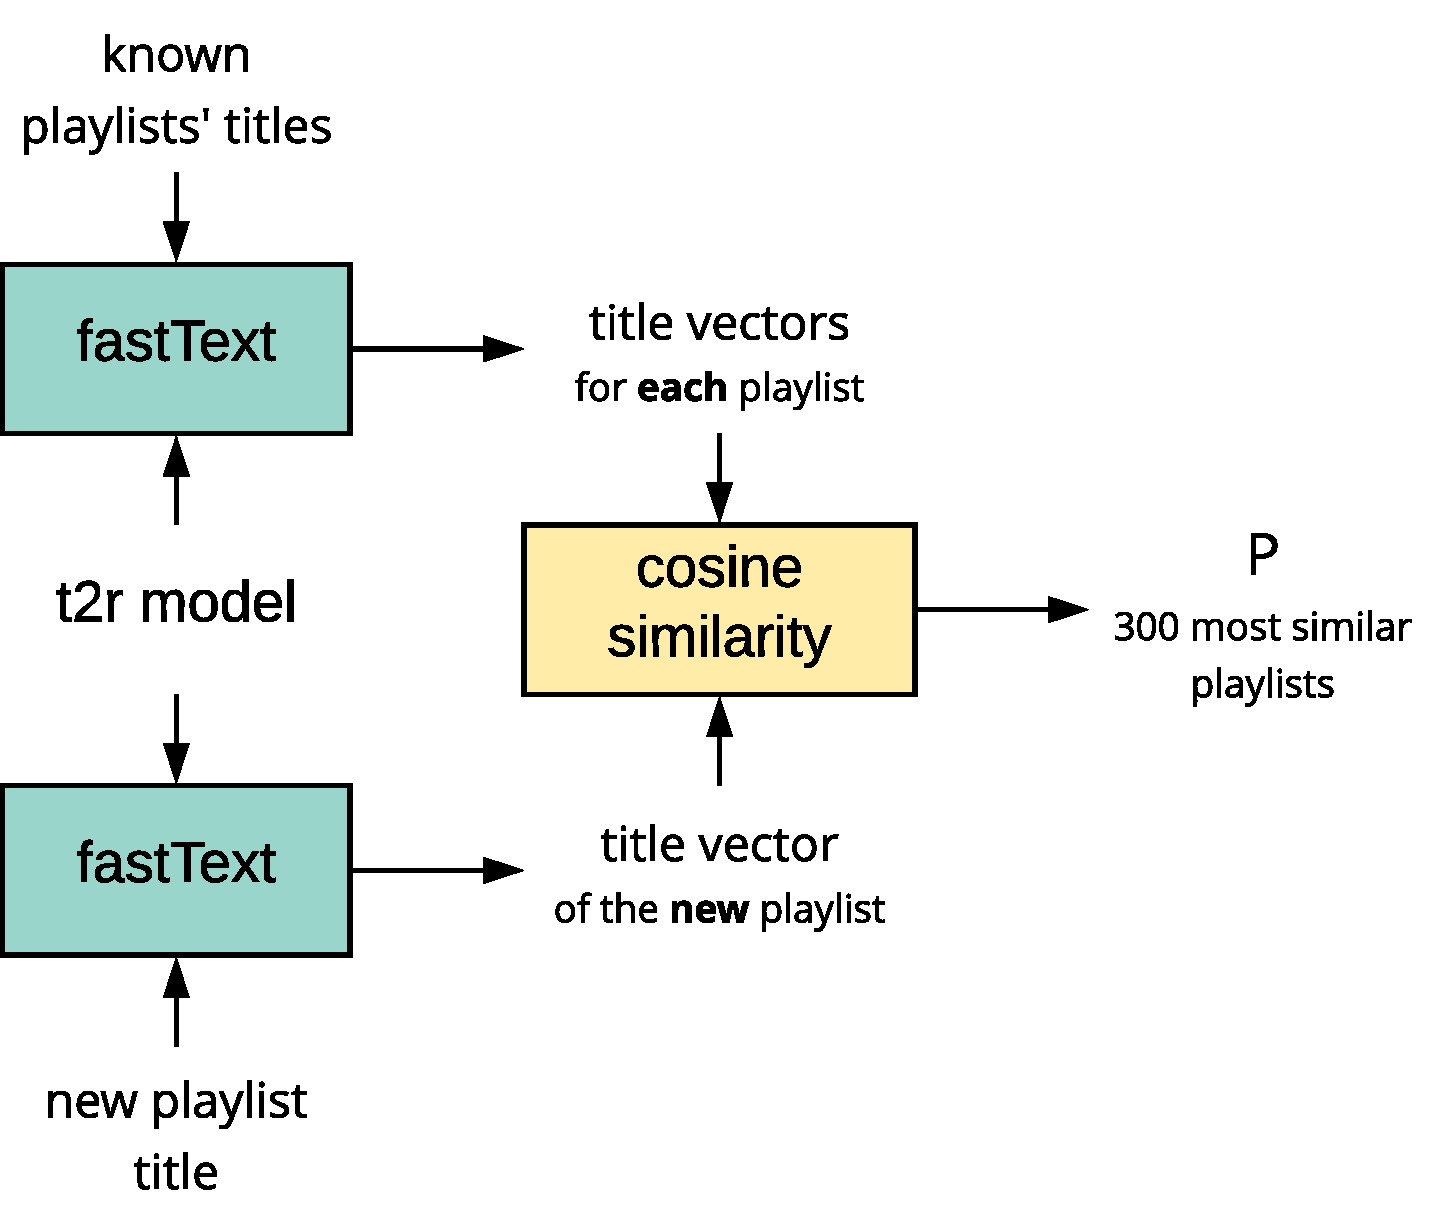
\includegraphics[width=\textwidth, width=0.4\textwidth]{figures/t2r_rec.pdf}
    \caption{The Title2Rec algorithm compares the fastText representation of the title of a seed playlist to the known ones using the cosine similarity.}
    \label{fig:t2r_rec}
\end{figure}
